\chapter{Extra Experimental Images}

\section{Pheromone Concentration Sensitibity}
\label{ap:exp-1}

\begin{figure}[H]
\myfloatalign
\subfloat[]
{\label{fig:ap-exp-a}
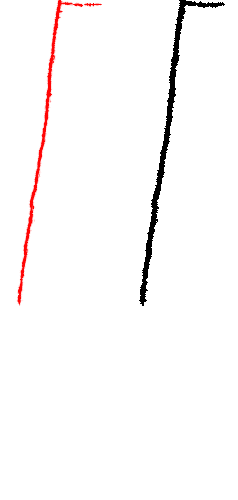
\includegraphics[width=.18\linewidth]{gfx/initial-extra-01}} \quad
\subfloat[]
{\label{fig:ap-exp-b}
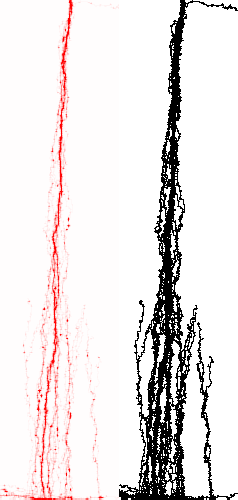
\includegraphics[width=.18\linewidth]{gfx/initial-extra-02}} \\
\subfloat[]
{\label{fig:ap-exp-c}
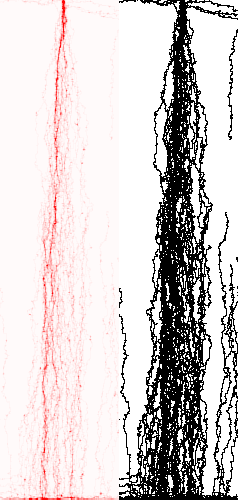
\includegraphics[width=.18\linewidth]{gfx/initial-extra-03}} \quad
\subfloat[]
{\label{fig:ap-exp-d}
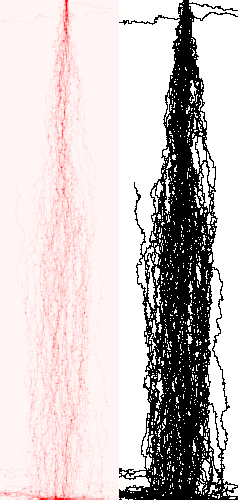
\includegraphics[width=.18\linewidth]{gfx/initial-extra-04}}
\caption{Full pheromone trail and space explored by the colony varying the initial concentration - 0.001 (a), 0.01 (b), 0.02 (c) and 0.04 (d).}\label{fig:ap-exp-01}
\end{figure}



\section{Forage radius investigation}
\label{ap:exp-2}

\begin{figure}[H]
  \centering
  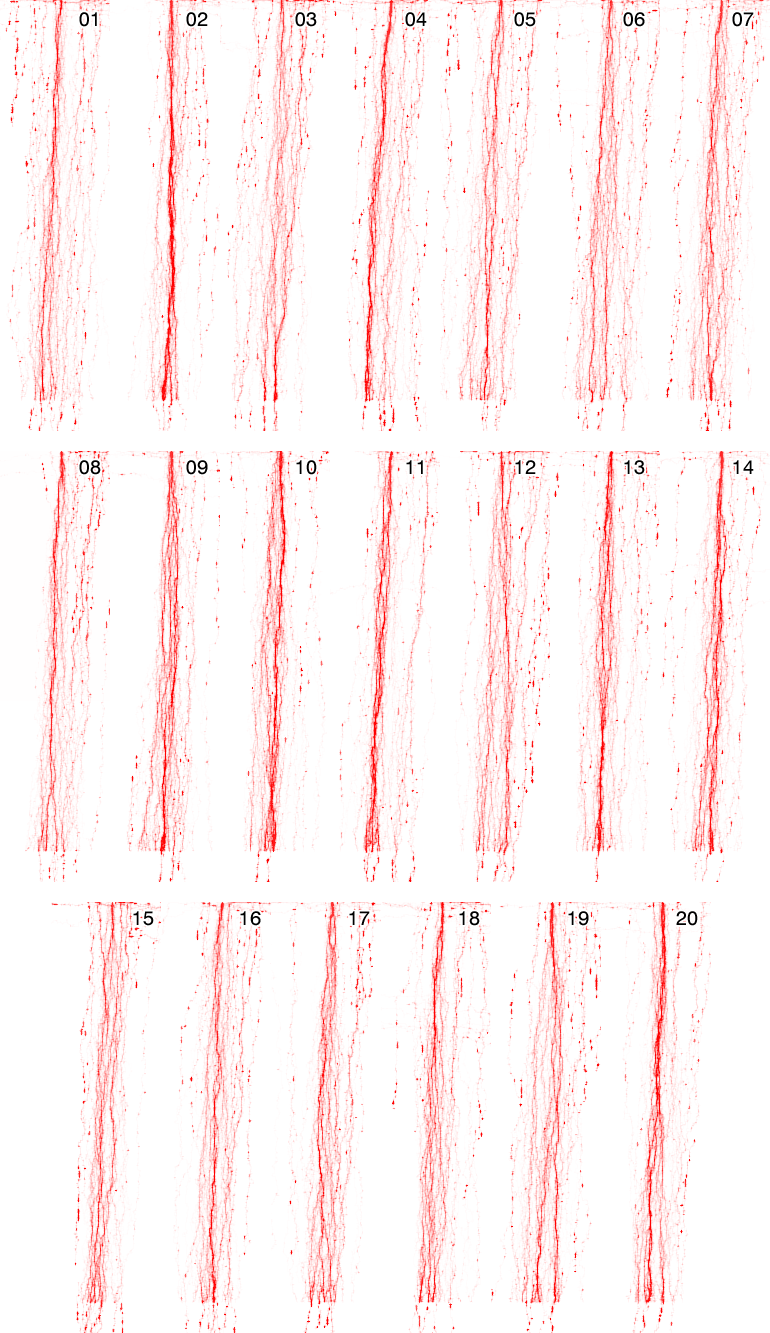
\includegraphics[width=0.75\linewidth]{gfx/radius-0-final.png}
  \caption{Full forage trails with radius at 0}
  \label{fig:radius-0-final}
\end{figure}

\begin{figure}[H]
  \centering
  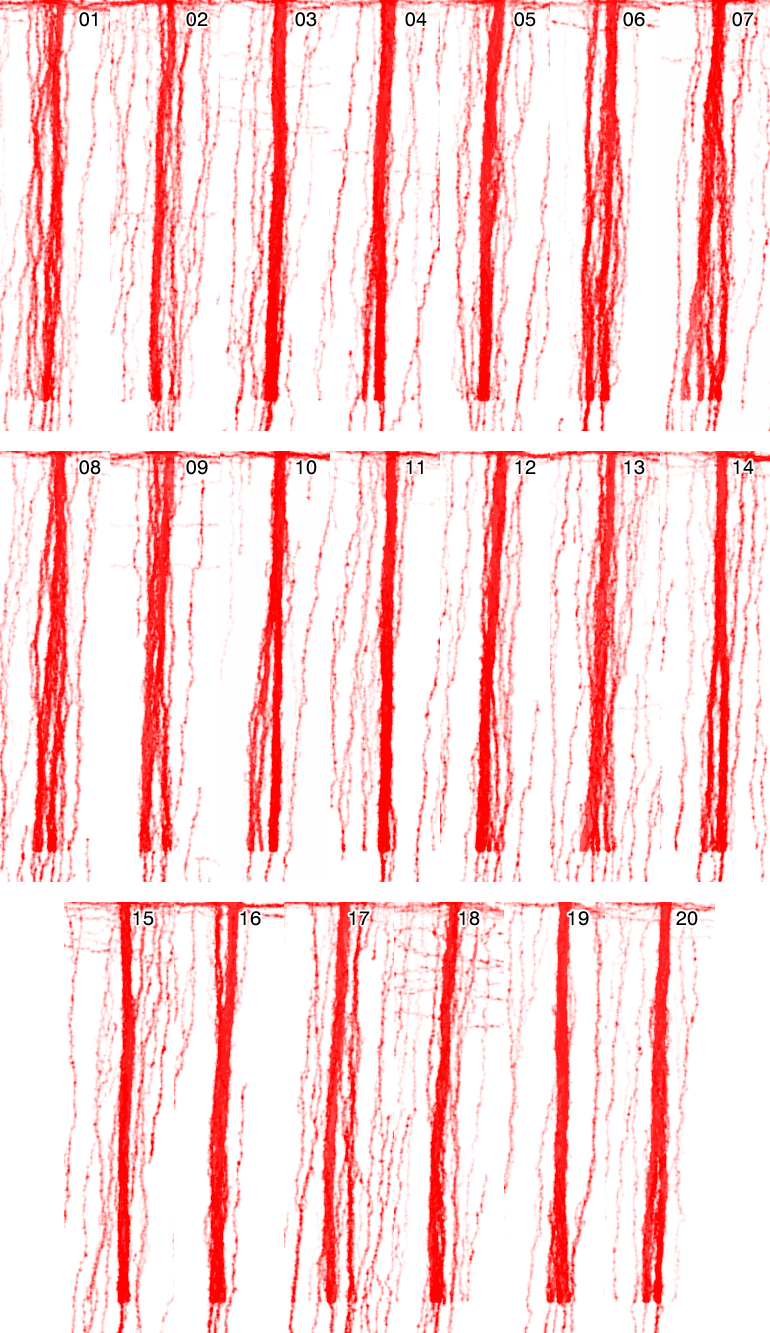
\includegraphics[width=0.8\linewidth]{gfx/radius-1-final.png}
  \caption{Full forage trails with radius at 1}
  \label{fig:radius-1-final}
\end{figure}

\begin{figure}[H]
  \centering
  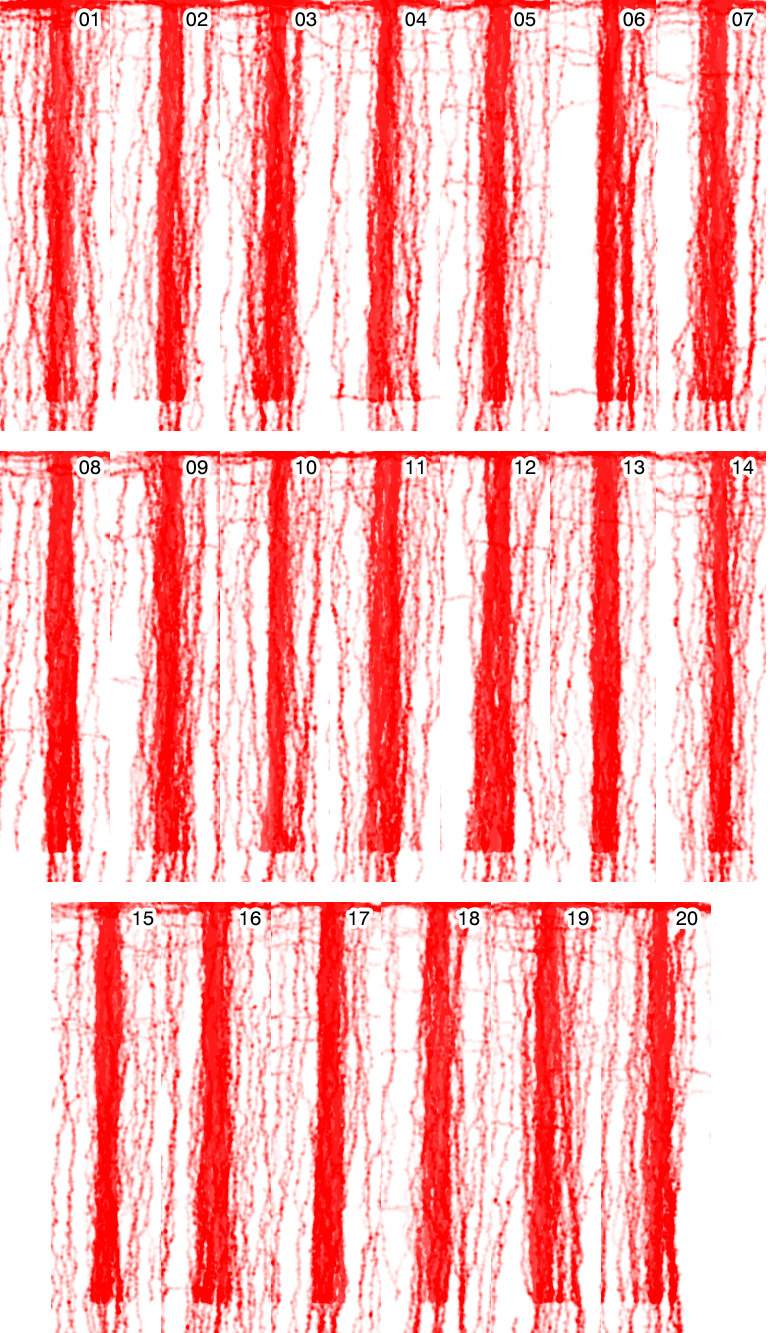
\includegraphics[width=0.8\linewidth]{gfx/radius-2-final.png}
  \caption{Full forage trails with radius at 2}
  \label{fig:radius-2-final}
\end{figure}